\documentclass[11pt]{article}
\usepackage[utf8]{inputenc}
\usepackage{lingmacros}
\usepackage{tree-dvips}
\usepackage{enumitem}
\usepackage{graphicx}
\usepackage{lmodern}
\usepackage[T1]{fontenc}
\usepackage[bottom]{footmisc}
\graphicspath{ {./images/} }

\newenvironment{remerciements}
  {
   \thispagestyle{empty}% no header and footer
   \vspace*{\stretch{1}}% some space at the top
   \itshape             % the text is in italics
  }
  {\par % end the paragraph
   \vspace{\stretch{3}} % space at bottom is three times that at the top
   \clearpage           % finish off the page
  }

\title{Monitoring des données BRAMS et détection automatique des échos de météore}
\author{Miguel Antoons}

\begin{document}

\begin{titlepage}
    \begin{center}
        
\includegraphics[]{logo_ephec.png}\\
        \Large
        \textbf{Technologie de l'Informatique}\\
        \large
        Avenue du Ciseau 15\\
        1348 Ottignies
    \end{center}

    \vspace*{\stretch{1.0}}

    \begin{center}
        \line(1,0){350}\\
        \LARGE\textbf{Monitoring des données BRAMS et détection automatique des échos de météore}\\
        \line(1,0){350}\\
        \vspace{0.5cm}
        \LARGE\textit{Miguel Antoons}\\
        \vspace{0.5cm}
        \Large\textbf{Rapporteur}\\
        \Large\textit{Monsieur Arnaud Dewulf}
    \end{center}

    \vspace{0.14cm}

    \begin{center}
        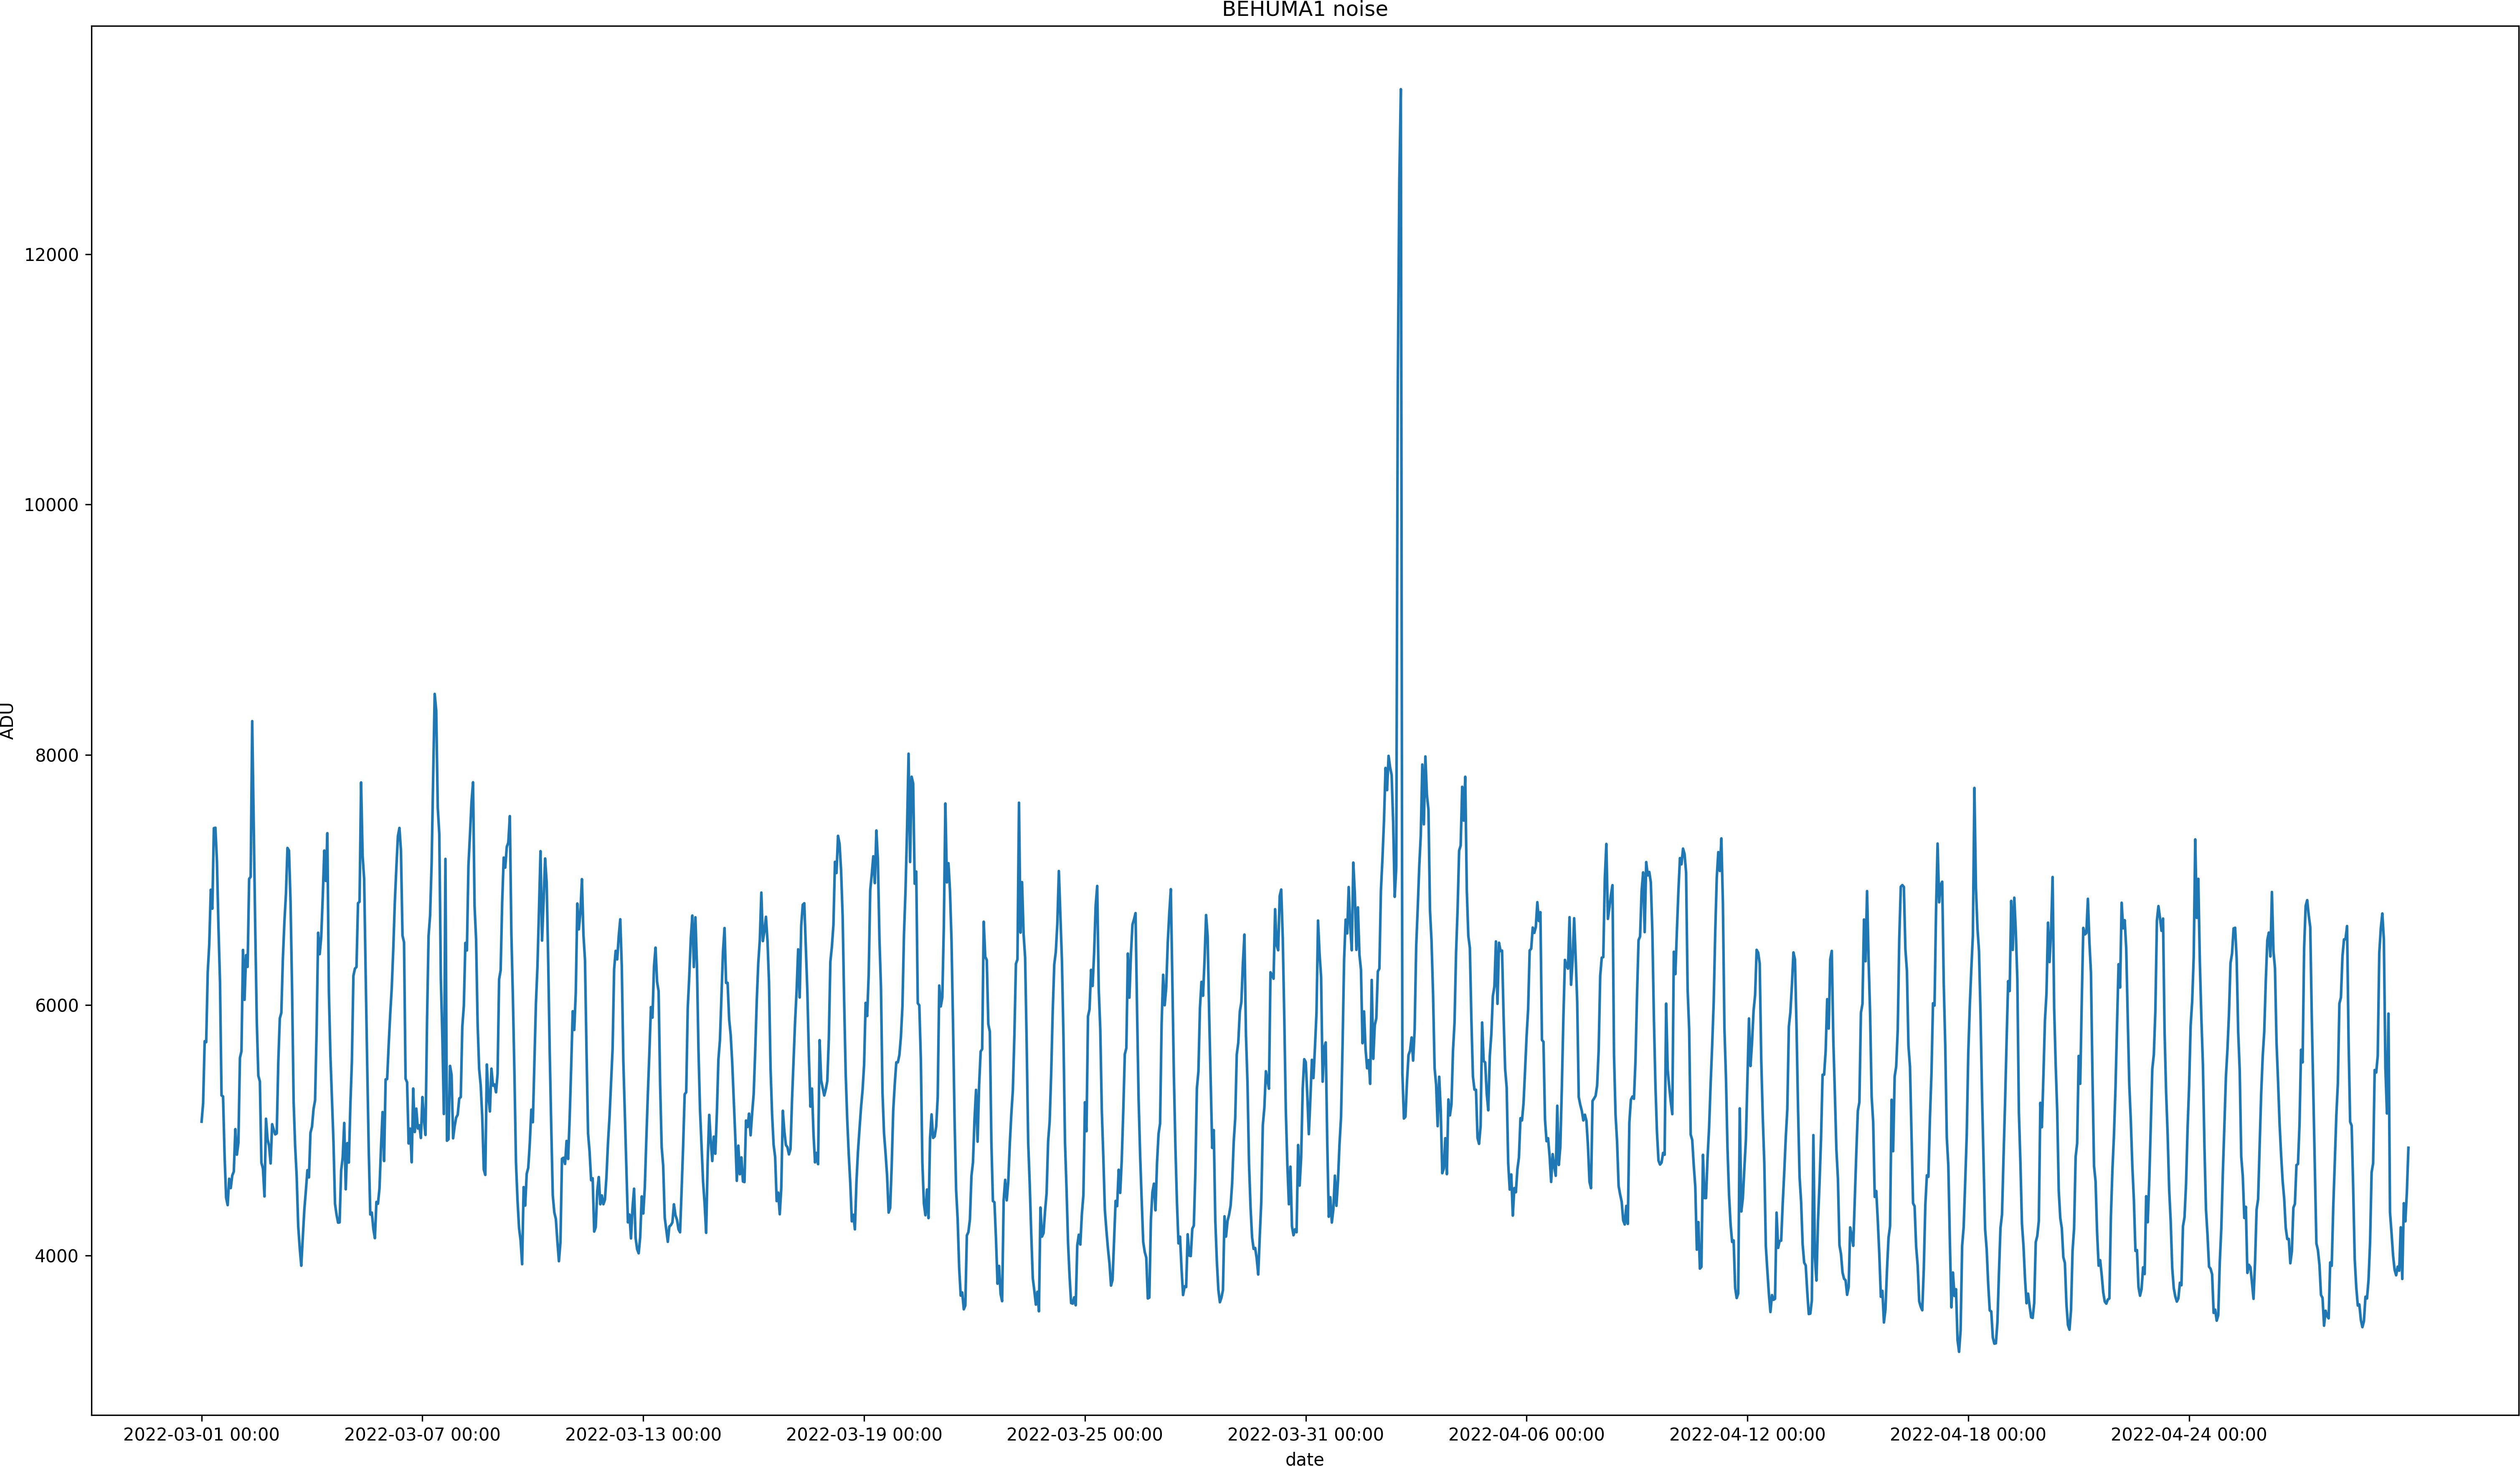
\includegraphics[scale=0.225]{page_garde.png}\\
        \vspace{0.14cm}
        \textit{2021-2022}
    \end{center}



    \vspace*{\stretch{2.0}}
\end{titlepage}

\section*{Remerciements}
\begin{remerciements}
    Je tiens tout d'abord à remercier toutes les personnes qui m'ont aidé à réaliser ce projet de fin d'études.\\
    \par
    En commençant par mon professeur rapporteur, à qui j'ai pu poser mes questions en cas de besoin et qui s'est assuré que tout se passe bien tout au long du projet.\\
    \par
    Ensuite, je voudrai remercier Mr Hervé Lamy pour avoir proposé ce sujet de fin d'études, mais également pour m'avoir expliqué, de façon claire et précise, toutes les notions qui nécessitaient des explications.\\
    \par
    Je tiens également à remercier Mrs Antoine Calegaro et Michel Anciaux, qui m'ont guidé quand c'était nécessaire et qui m'ont conseillé durant le projet de fin d'études.\\
    \par
    Enfin, je voudrais exprimer ma reconnaissance envers toutes les personnes qui m'ont conseillé sur, et ont relu ce rapport de projet de fin d'études.
\end{remerciements}

\newpage

\tableofcontents

\newpage

\section{Introduction}

\subsection{Le projet BRAMS}

Lancé en 2010 par Monsieur Hervé Lamy à l'Institut Royal d'Aéronomie Spatiale de Belgique, le projet BRAMS (Belgian RAdio Meteor Stations) à pour but de collecter et stocker des données relatives à des objets rentrant dans l'atmosphère belge et, plus précisément, des météores.
Ces données pourront ensuite être analysés afin de retrouver la trajectoire, la vitesse ou encore la masse d'un ou de plusieurs météores.\\

\subsubsection{Le Réseau BRAMS}

Afin d'accomplir ce but, le projet BRAMS dispose d'un réseau de stations nommé le réseau BRAMS.
Ce réseau est composé d'un ensemble de quarante-deux stations émettrices, situées en Belgique ou dans les pays avoisinants, et d'un émetteur dédié situé à Dourbes, dans le sud de la Belgique.\\
\\
Il existe 2 types de station de réception :
\begin{itemize}
    \item Il y a d'abord les stations avec des récepteurs Icom IC-R75, que j'apellerai les récepteurs ICOM dans ce document.
          Ce sont les premières stations réceptrices mises en service pour le réseau BRAMS.
          Actuellement, ces stations ne sont plus utilisées suite à l'arrêt de la commercialisation du récepteur Icom IC-R75.
          De plus, une variation de température pouvait causer une légère déstabilisation en fréquence.
    \item C'est alors que les stations utilisant le récepteur RSP 2 ont été développés.
          Ces stations n'éliminaient pas seulement en grande partie les problèmes des anciennes stations, mais sont également plus compacts et plus faciles à installer.
          Une image des stations RSP 2 peut être trouvé à la figure 1.
\end{itemize}

\begin{figure}[t]
    \begin{center}
        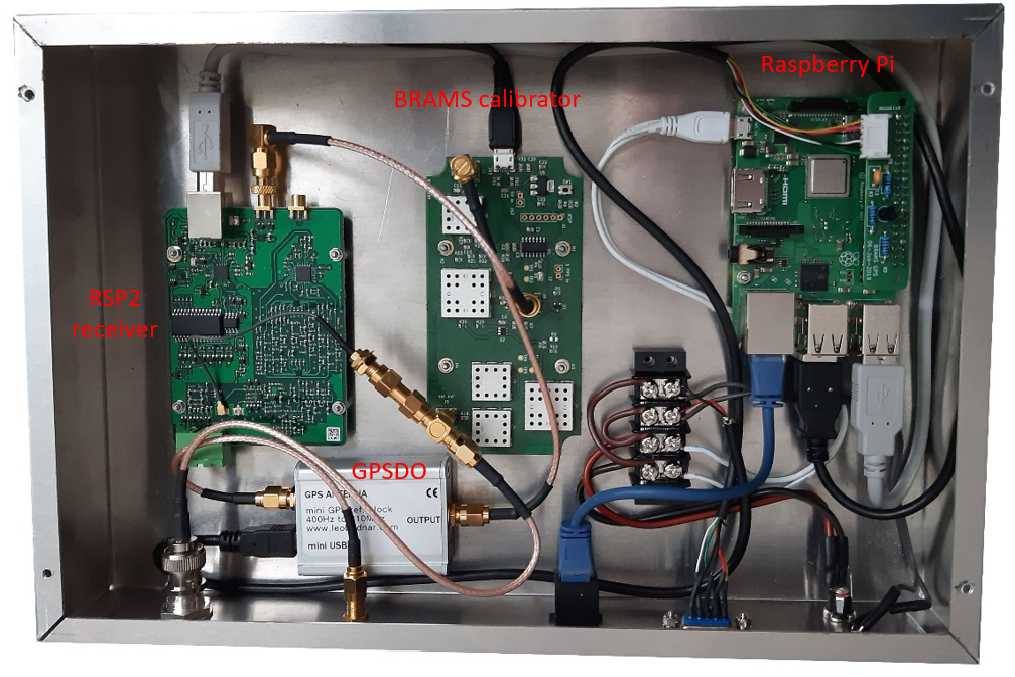
\includegraphics[scale=0.5]{RPS2.png}
        \caption{Station RSP 2 du réseau BRAMS}
    \end{center}
\end{figure}

\subsubsection{Le Format WAV}

% ! corrections for chunkSize and subChunkSize

Le format de fichier WAV (Waveform Audio File) est un format destiné au stockage de signal audio développé par Microsoft et IBM.
Il est construit conformément au RIFF (Ressource Interchange File Format) ce qui veut dire que le fichier est organisé en blocs de données, aussi nommés des "chunks" ou "data chunks".\\
\\
Chaque bloc de données dispose d'un ID codé sur 4 octets, qui représente souvent un mot de 4 lettres.
Suit ensuite le champ "ChunkSize" indiquant la taille des données à venir dans l'ensemble du fichier, codé également sur 4 octets.
Cette valeur exclut donc les champs "ID" et "ChunkSize" ainsi que la taille de tous les éventuels blocs de données venant avant le bloc courant.
Après ces 2 champs, on est libre de rajouter le nombre de champs que l'on souhaite, avec la taille en octets que l'on souhaite.\\
\\
Pour un fichier WAV, on retrouve typiquement 3 blocs de données.
On retrouve premièrement le bloc "RIFF" qui contient la taille de l'entièreté du fichier moins 8 octets (4 octets du champ "ID" et 4 octets du champ "ChunkSize") suivi du champ indiquant le format du fichier.
Dans le cas du fichier WAV, ce dernier contient les quatre lettres "WAVE".\\
\\
Le deuxième bloc, nommé le bloc FMT\footnote{FMT pour format}, contenu dans un fichier WAV ordinaire contient toutes les données techniques des données.
On y trouve notamment la fréquence d'échantillonnage, le nombre de pistes audio ou encore le nombre d'octets par secondes.\\
\\
Vient enfin le bloc principal du fichier : le bloc de données.
C'est dans ce bloc que se trouvent les données audio brutes.
La taille de ce bloc varie bien-entendu selon les caractéristiques techniques des données audio (longueur, fréquence d'échantillonnage, nombre de pistes, etc.).\\
\\
Une chose à noter à propos des fichiers WAV est que leur structure offre une grande flexibilité.
En effet, elle permet non-seulement de lire et interpréter les fichiers facilement, mais également de rajouter des blocs de données personnalisés sans corrompre les autres données.\\
\\
La figure 2 montre la structure d'un fichier WAV ordinaire.

\begin{figure}[t]
    \begin{center}
        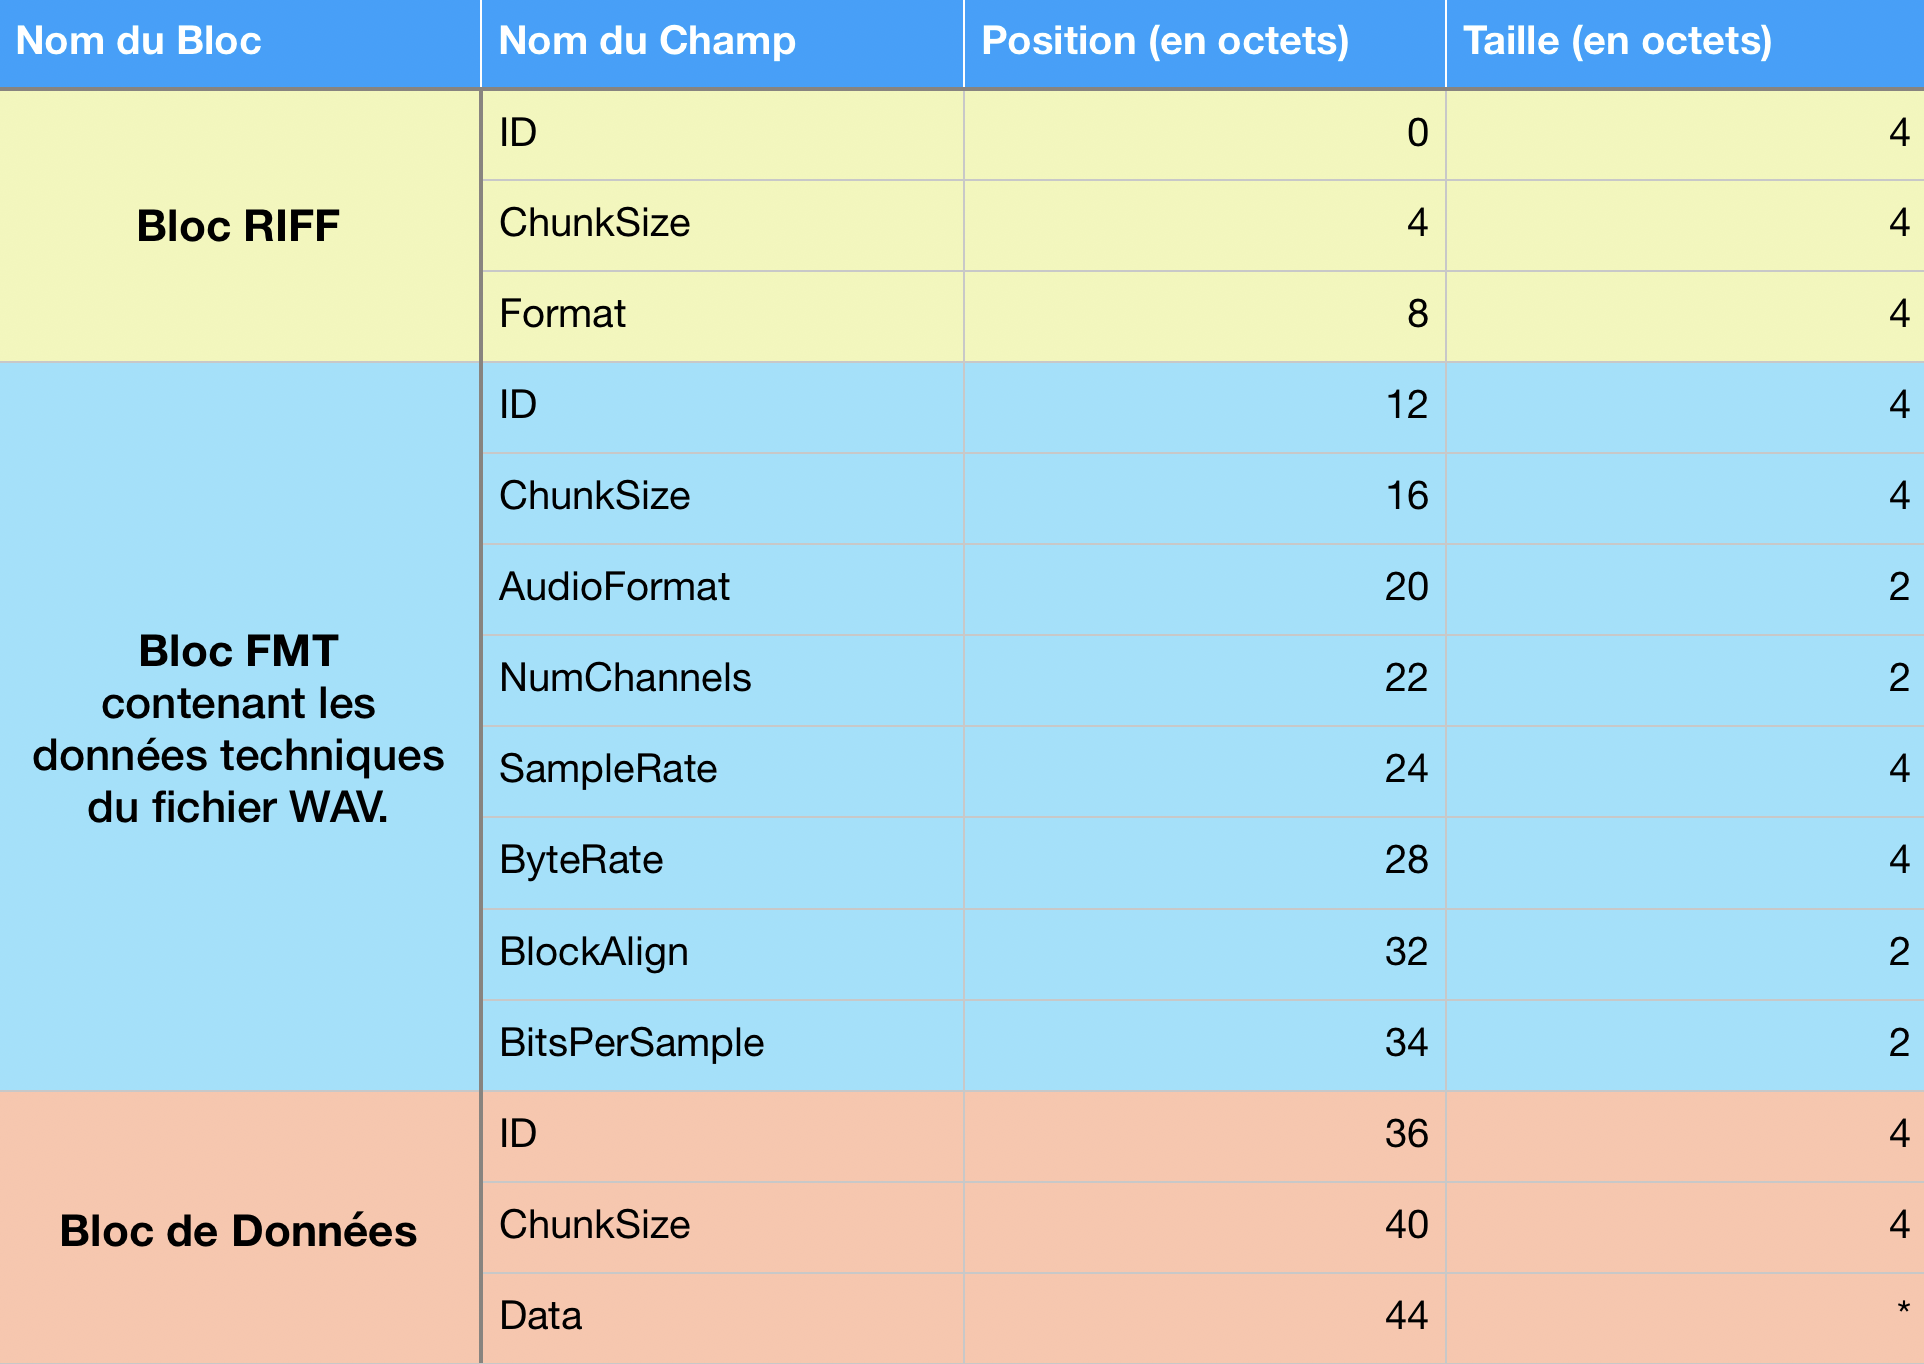
\includegraphics[scale=0.3]{wav_structure.png}
        \caption{Structure d'un fichier WAV ordinaire}
    \end{center}
\end{figure}

\newpage

\subsubsection{La Réflexion Spéculaire}

Pour comprendre le fonctionnement du réseau BRAMS, la première chose à savoir est : lorsqu'un météore passe dans l'atmosphère, il laisse derrière lui une trainée ionisée.
Cette trainée à la propriété de réfléchir les ondes radio.
Dans la plus grande partie des cas cette réflexion se fait en un seul point le long de la trajectoire, phénomène qui s'appelle la réflexion spéculaire (illustré à la figure 3).
La position de ce point, nommé le point de réflexion spéculaire, dépend notamment du positionnement de l'émetteur, du positionnement du récepteur et de la trajectoire du météore.\\
\\
Pour exploiter le phénomène de la réflexion spéculaire et réussir à détecter les météores à l'aide d'ondes radios, le réseau BRAMS fonctionne de la façon suivante :
\begin{enumerate}
    \item Un émetteur, situé à Dourbes, transmet de façon continue un signal à une fréquence de 49.97 MHz.
          Ce signal est émis en direction du ciel et peut être réfléchi sur des trainées ionisées dans le sillage des météores.
    \item Lorsque le signal est réfléchi, il peut être détecté par une ou plusieurs stations réceptrices faisant partie du réseau BRAMS.
          Un signal calibreur est alors additionné au signal venant du ciel.
          Ce signal est injecté à 49.9705 MHz, c'est-à-dire 500 Hz plus haut que le signal direct.
          Il dispose d'une amplitude fixe et sert de référence d'amplitude pour le reste du signal.
          La station réceptrice décale ensuite le signal direct de 49.97 MHz vers une fréquence de 1 kHz.
    \item Ensuite, la station réceptrice enregistre l'ensemble du signal dans un fichier audio de type WAV.
          Le signal est échantillonné à une fréquence de 5512,5 Hz pour les stations ICOM et 6048 Hz pour les stations RSP2.
          Si tout se passe bien, un fichier est généré toutes les cinq minutes et chaque fichier devrait commencer et terminer à un temps prédéfini (par exemple : 16 h 00 à 16 h 05, 16 h 05 à 16 h 10, etc.).
    \item Tous les fichiers générés par les stations réceptrices sont envoyés à intervalle régulier aux serveurs utilisés pour le projet BRAMS par internet.
    \item Une fois sur le serveur, les fichiers WAV sont archivés, manipulés et étudiés par les scientifiques du projet BRAMS afin d'en extraire les informations utiles.
\end{enumerate}

\begin{figure}[t]
    \begin{center}
        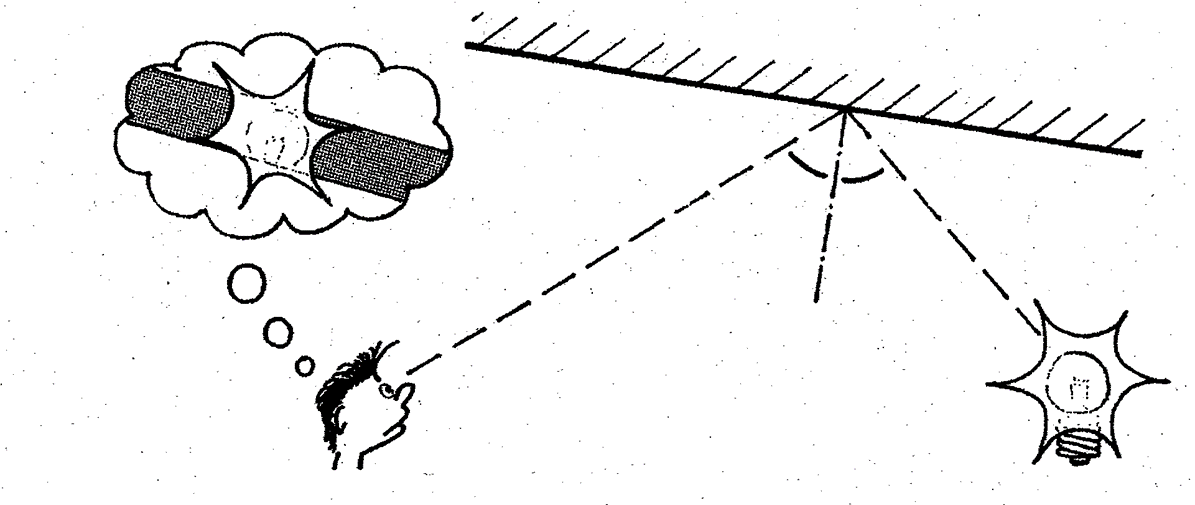
\includegraphics[scale=0.6]{SpecularReflection.png}
        \caption{Représentation de la réflexion spéculaire.}
    \end{center}
\end{figure}

\subsubsection{Les Données BRAMS}

Un fichier WAV venant d'une station réceptrice contient donc le signal capté par l'antenne ensemble avec un signal calibreur.
Il est composé d'une seule piste audio, échantillonnée à une fréquence de 5512.5 Hz ou 6048 Hz.
Cette fréquence permet d'enregistrer des données dans une bande de fréquences allant jusqu'à 2756.25 Hz ou 3024 Hz (ou la moitié de la fréquence d'échantillonnage), selon le théorème de Nyquist.
Sachant que les échos de météores apparaissent typiquement dans une bande de fréquence de 100 Hz autour du signal de l'émetteur à 1000 Hz, cette bande de fréquence couvre l'ensemble des signaux utiles à l'étude des météores.\\
\\
À chaque fichier WAV est rajouté un bloc de données (data chunk) conçu pour faciliter l'étude des données.
Dans ce bloc, on retrouve quelques informations relatives à la station de réception, la station émettrice, le signal GPS\footnote{Global Positioning System} ou encore, la fréquence d'échantillonnage.
Ce bloc de données se trouve entre le bloc FMT et le bloc de données.\\
\\
Ces fichiers audio, comme montrée à la figure 4, sont très difficiles à interpréter.
Ils sont composés de bruits et de parasites sur l'entièreté de leur bande de fréquence.
Par contre, lorsque l'on calcule le spectrogramme du fichier WAV, les données deviennent beaucoup plus simples à lire.
\begin{figure}[t]
    \begin{center}
        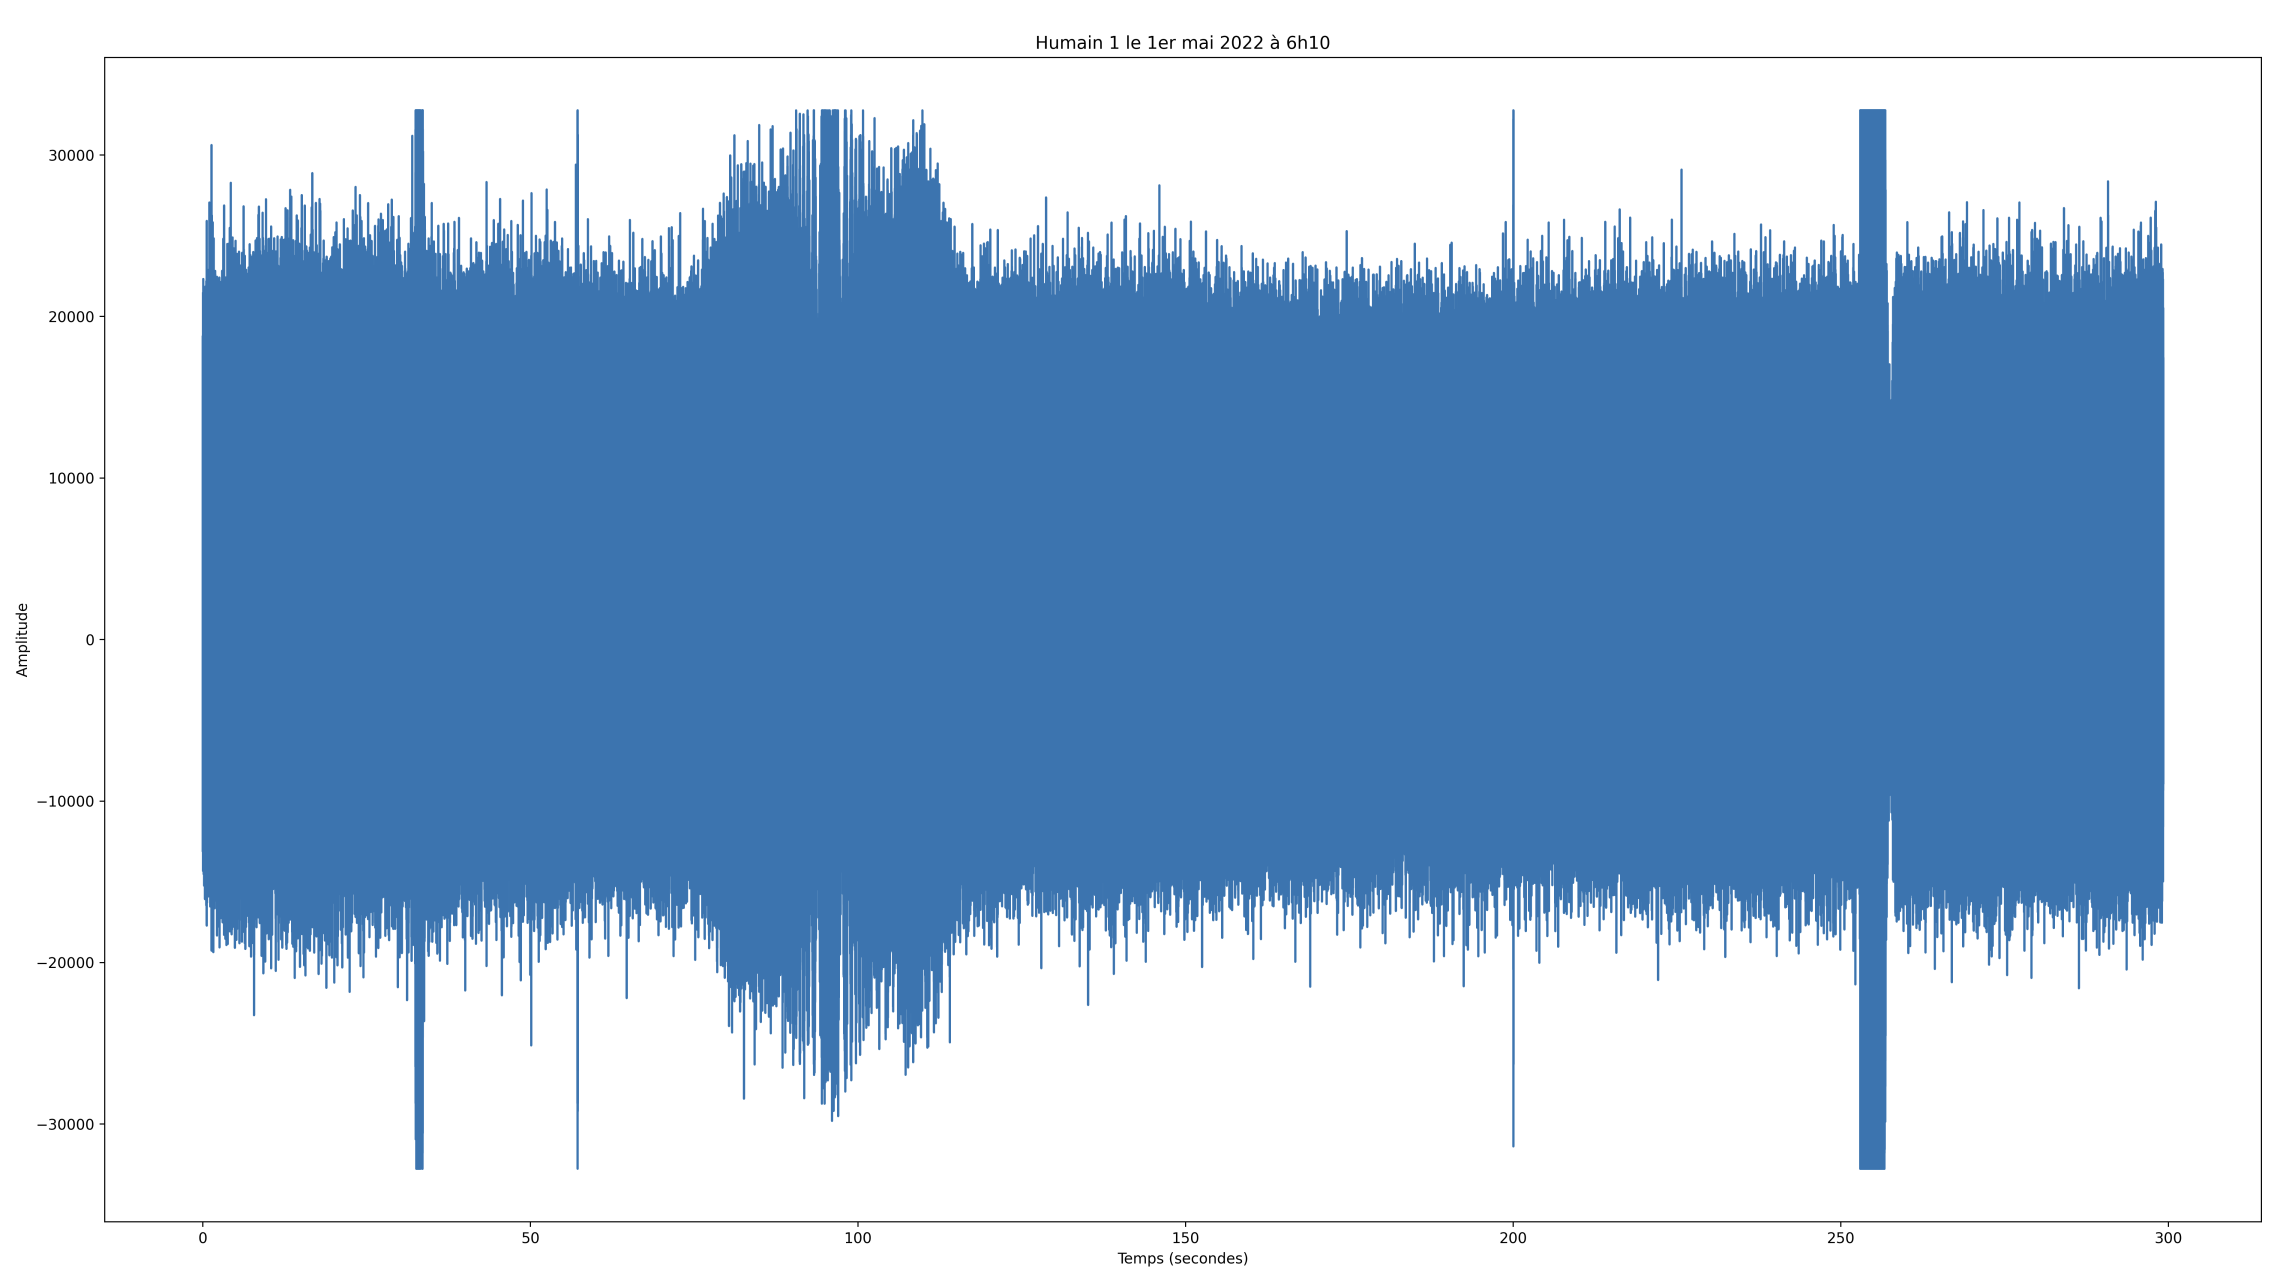
\includegraphics[scale=0.5]{wav_brut.png}
        \caption{Données brutes venant d'un fichier audio d'une station réceptrice.}
    \end{center}
\end{figure}
\\
\\
Un spectrogramme est une représentation différente des données contenues dans un fichier audio.
Au lieu de représenter la puissance sur l'ordonnée et le temps sur l'abscisse, un spectrogramme représente la répartition des fréquences au cours du temps.
Il contient donc trois axes :
\begin{itemize}
    \item Sur l'abscisse on retrouve toujours le temps.
    \item Sur l'ordonnée on retrouve la fréquence.
    \item Sur la cote, on retrouve la puissance. Cet axe est souvent représenté par un code couleur.
\end{itemize}

Pour générer un spectrogramme, il faut calculer un ensemble de Transformées de Fourrier.
La Transformée de Fourrier permet de représenter la répartition de puissance entre les fréquences contenues dans un signal ou une partie d'un signal temporel.
Elle produit donc se qu'on appelle le spectre du signal.
Elle se calcule sur un nombre quelconque d'échantillons qui se suivent dans un signal temporel.
Dans l'informatique, elle est souvent calculée à l'aide de la FFT\footnote{Faste Fourier transform}.
C'est un algorithme qui permet de calculer une Transformée de Fourrier plus rapidement, mais qui exige un nombre d'échantillons $2^{n}$.\\
\\
Sur la figure 5, on peut voir en rouge un signal temporel et le spectre de ce même signal en bleu.
Les signaux en mauve claire sont les signaux à une fréquence, dont le signal rouge est composé.
\begin{figure}[t]
    \begin{center}
        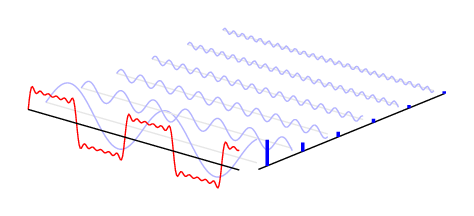
\includegraphics[scale=0.7]{spectre.png}
        \caption{Représentation visuelle de la Transformée de Fourier.}
    \end{center}
\end{figure}
\\
\\
Dans le cas des spectrogrammes pour le projet BRAMS, les FFT contenus dans un spectrogramme sont calculés sur 16384 échantillons.
Si on suppose qu'un fichier WAV venant d'une station réceptrice dure en moyenne trois-cents secondes (ou cinq minutes), un spectrogramme est composé d'environ 101 spectres pour les stations ICOM et 111 pour les staions RSP2.
Ce nombre est obtenu avec la formule ci-dessous, où Fs est la fréquence d'échantillonnage, T la durée en secondes du signal et nfft le nombre d'échantillons utilisés pour générer un spectre.
\[\frac{Fs * T}{nfft}\]
Le spectrogramme généré aura une résolution fréquentielle, donnée par la formule \(Fs / nfft\), de 0.34 Hz pour les stations ICOM et 0.37 Hz pour les stations RSP2.
Sa résolution temporelle, donnée par la formule \(nfft / Fs\), est de 2.97 secondes pour les stations ICOM et de 2.7 secondes pour les stations RSP2.
Un exemple de spectrogramme venant d'une station de réception est affiché à la figure 6.

\begin{figure}[t]
    \begin{center}
        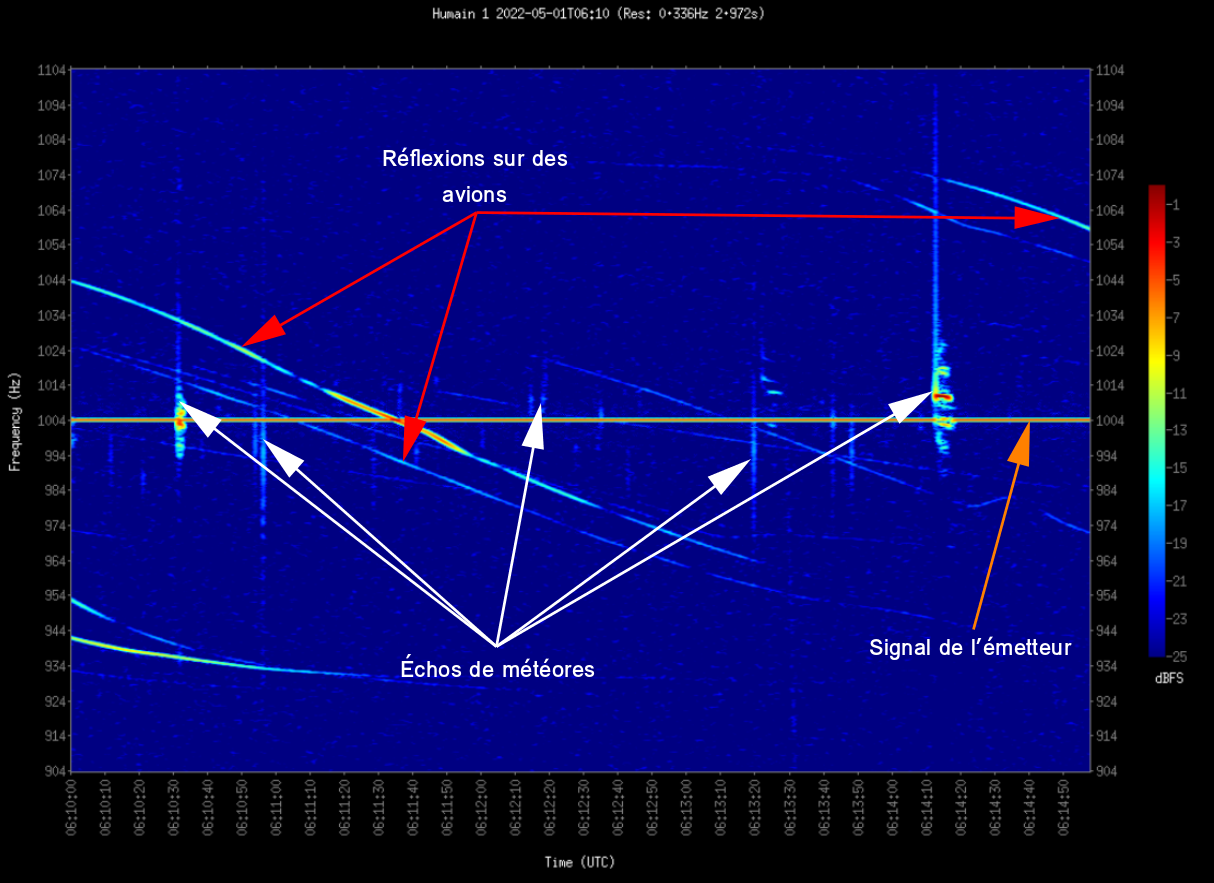
\includegraphics[scale=0.29]{spectrogramme_legend.png}
        \caption{Exemple d'un spectrogramme du projet BRAMS.}
    \end{center}
\end{figure}

\subsubsection{L'Archive BRAMS}

Quand les fichiers venant des stations de réception sont archivés, ils sont placés dans une structure de répertoires spécifique.
Cette structure dépend de la date de début d'enregistrement des données contenues dans le fichier.\\
\\
Dans la première couche de l'archive, on retrouve un répertoire par station BRAMS.
Chaque nom de répertoire est le code de location de la station dont elle contient les données.
Ensuite, on retrouve un nombre de répertoires, chacun contenant les fichiers d'une année spécifique.
Le nom de ces répertoires est donc l'année des données qu'elles contiennent.
Si on rentre dans le répertoire d'une année, on se retrouve dans la troisième couche de l'archive BRAMS.
Ici, les données sont encore une fois séparées selon le mois d'enregistrement du fichier.
Finalement, dans la quatrième couche de l'archive, on retrouve un répertoire par jour d'enregistrement d'un fichier.\\
\\
Dans chaque répertoire représentant un jour spécifique, on retrouve les données BRAMS organisés par heure dans des fichiers de format tar.
Ce format permet de regrouper plusieurs fichiers dans un même fichier, qui prend alors le format tar.
Le nom des fichiers tar et les fichiers wav qui se trouvent à l'intérieur des fichiers tar suivent également une structure fixe.
Il est composé de six informations ordonnées de la manière suivante :
\begin{enumerate}
    \item Les trois lettres \textbf{RAD}.
    \item Le code de la station émettrice.
          Comme il n'y a qu'une station réceptrice à présent, la valeur sera toujours \textbf{BEDOUR}.
    \item La date du début de l'enregistrement du fichier.
          Elle respecte le format YYYYMMDD.
    \item Le temps du début de l'enregistrement du fichier, précis à la minute.
          Elle respecte le format HHMM.
    \item Le code de location de la station émettrice.
          Un code de location est composé de deux informations.
          Les deux premiers caractères représentent le code du pays ou se trouve la station (e.g. BE, FR, ...) et les quatre lettres restantes représentent typiquement les quatre premières lettres de la ville où est situé la station (e.g. HUMA pour Humain, UCCL pour Uccle, ...).
    \item L'alias de la station.
          Elle est composée des trois caractères 'SYS', suivie du numéro de l'antenne qu'a capté les données.
          Le numéro de l'antenne est toujours écrit sur trois chiffres (e.g. 001, 002, ...).
\end{enumerate}

Toutes ses valeurs sont séparées par un tiret bas.
Un exemple de nom de fichier est affichée à la figure 7.

\begin{figure}[t]
    \begin{center}
        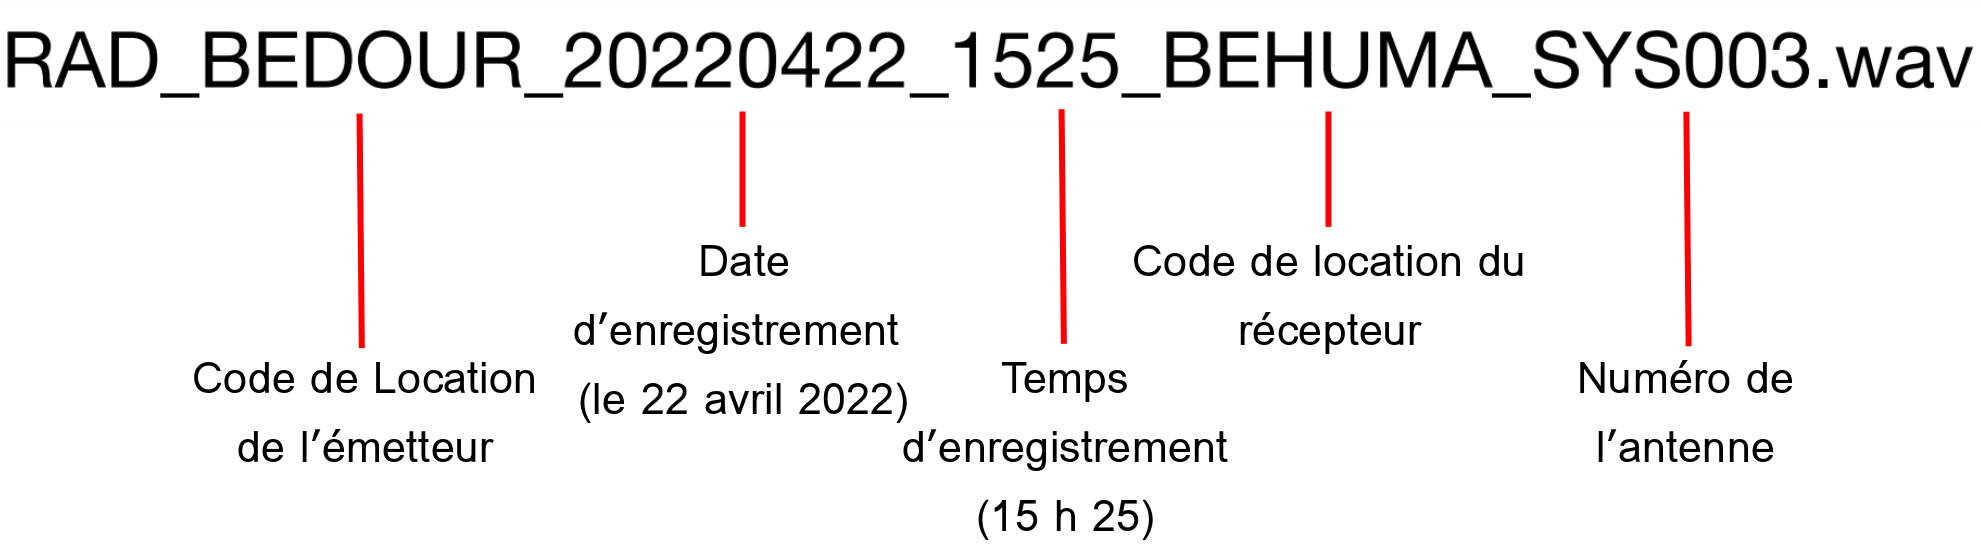
\includegraphics[scale=0.15]{file_name.png}
        \caption{Exemple de nom de fichier BRAMS.}
    \end{center}
\end{figure}

\newpage

\subsection{Problématique liée à l'étude des données BRAMS}

Afin de pouvoir trouver la trajectoire d'un météore dans l'atmosphère, il est nécessaire de rechercher par quelles stations réceptrices le météore est détecté.
Ceci est une procédure qui prend un temps non négligeable pour les scientifiques du projet.
En effet, toutes les stations de réception ne détectent pas tous les météores.
De plus, certaines données peuvent être corrompues ou encore, non-existantes.\\
\\
De plus, savoir, ou au moins avoir une idée, si un météore détecté par une station réceptrice est le même qu'un météore détecté sur une autre station réceptrice serait une grosse économie de temps.\\
\\
C'est pour cette raison que les membres du projet BRAMS souhaitent disposer d'un programme qui remplit deux fonctions.
D'une part, elle doit être capable de vérifier si un fichier contient des données non-corrompues et utilisables.
D'autre part, elle devra, sur base d'un écho de météore d'une station de réception, retrouver les échos de ce même météore sur des fichiers d'autres stations de réception.

\newpage

\section{Méthodologie}

Afin d'arriver à un résultat final de qualité et qui est conforme aux requis des membres du projet BRAMS, il est important d'utiliser une bonne méthodologie.\\
\\
La première chose que j'ai fait est : comprendre quoi exactement le programme devrait faire.
Pour ce faire, plusieurs réunions ont eu place avant la réalisation du travail.
Durant ces réunions, j'ai pu poser mes questions et demander des explications sur les concepts à connaître pour pouvoir réaliser le travail.
Ayant reçu des documents qui expliquent de façon claire et précise le fonctionnement du réseau BRAMS, j'ai pu me préparer avant de m'attaquer à l'analyse et la réalisation du travail.\\
\\
Durant la période d'analyse et de réalisation du TFE, j'ai pu régulièrement demander validation quant à la direction que je prenais pour mon travail.
Je présentais régulièrement mes réalisations aux scientifiques du projet BRAMS afin d'avoir un feedback régulier et de pouvoir perfectionner mon programme un maximum.\\
\\
Dans le but d'être plus efficace lors de l'écriture des fonctionnalités pour le programme, je décrivais avant ce que cette fonctionnalité devait faire.
Ensuite, je la divisais en tâches techniques afin de pouvoir m'organiser plus facilement.
Chaque tâche technique contenait et expliquait les étapes que le programme devrait exécuter pour accomplir cette tâche technique.
Les étapes étaient décrites textuellement, par pseudo-code, par schéma ou encore, par le mélange de deux ou trois des moyens cités.\\
\\
Durant l'entièreté du projet de fin d'études, j'ai tenté de garder un rythme de travail régulier.
Je me suis organisé de telle façon de pouvoir travailler une moyenne de 23 heures par semaine.
Une grande partie de ces heures se sont déroulés lorsque je rentrais de mon stage ou pendant le week-end.\\

\newpage

\section{Technologies utilisées}

\subsection{Python}

Le programme réalisé est entièrement écrit en Python.
Ce choix a été pris premièrement pour les librairies performantes et open-source qu'offre Python.
En effet, des librairies comme numpy, scipy ou encore matplotib ont été très utiles pour arriver à un résultat performant et fonctionnelle.
Ces librairies offrent beaucoup de flexibilité et offrent une haute performance grâce à leur écriture en C, C++ et même en Fortran.\\
\\
Un autre avantage du Python est sa portabilité.
Puisque c'est un langage interprété, largement répandu, quasiment tous les systèmes d'exploitation le supportent.
Ceci a facilité aussi bien la phase de développement que la phase de testing du projet de fin d'études.\\
\\
Un des désavantages souvent évoqués pour Python, est que le langage est lent pour des gros traitement de données.
Cependant, dans le cas de ce travail, ceci ne fut pas un problème et les librairies utilisées étaient largement assez rapide.
Ceci est dû, entre autres, grâce à la nature open-source de ces librairies ainsi que leur âge.
Suite à ces deux facteurs, des milliers de personnes travaillent sur ces librairies depuis plusieurs années dans le but d'optimiser le plus possible ses fonctions et méthodes.

\subsection{MariaDB}

Afin de sauvegarder les données produites par le programme, une base de données est requise.
Les données produites seront toutes liées à un fichier, le choix d'une base de données relationnelle est donc appropriée.\\
\\
MariaDB est une dérivée de MySQL.
Elle a l'avantage d'être gratuite et open-source.
Grâce à une large communauté contribuant au développement continu de MariaDB, elle est souvent plus performante que MySQL.
De plus, étant open-source, les problèmes sont résolus rapidement par des mises à jour régulières.\\
\\
Enfin, le projet BRAMS dispose actuellement déjà d'une base de données MariaDB.
Elle contient, entre autres, les données de chaque fichier archivé, venant d'une station de réception BRAMS.
Pour le programme, il suffit donc de rajouter les champs nécessaires à la table contenant les fichiers.
MariaDB est donc le choix logique.

\newpage

\section{Lecture des Fichiers BRAMS}

Avant de commencer à développer des outils pour la détection des météores ou pour l'analyse des fichiers BRAMS, il a fallu développer un logiciel permettant de lire ces fichiers.
Ce logiciel sera implémenté dans un module Python contenant une classe nommée BramsWavFile.
Ceci veut dire qu'il pourra facilement être utilisé par d'autres fichiers Python et qu'il doit donc être flexible.
Dans cette section, le fonctionnement de ce module est expliqué en détail.

\subsection{Librairies Utilisées}

\subsubsection{Os}

La librairie os de Python contient une suite de fonctions permettant d'interagir avec le système d'exploitation.
Cette librairie vient par défaut avec une installation de Python, ce qui évite de devoir l'installer lorsque nécessaire.
Pour la classe BramsWavFile, la librairie os sera utilisée afin de récupérer des chemins de dossiers et fichiers, et pour récupérer le contenu d'un dossier.

\subsubsection{Numpy}

Numpy est une librairie Python utilisée lorsqu'on travaille avec des listes très larges.
Il contient de nombreuses fonctions pour l'algèbre linéaire, les Transformées de Fourier et les matrices.
Par rapport aux listes classiques de Python, les listes Numpy (aussi appelés des ndarray) sont beaucoup plus rapides.\\
\\
Ceci est dû à trois raisons principales.
La première est que les listes Numpy sont stockés à un endroit continu dans la mémoire RAM\footnote{Random Access Memory}, ce qui permet un accès et une manipulation plus efficace des données.
Ensuite, comme Numpy est une librairie open-source, il est continuellement adapté à des nouvelles architectures de processeurs.
Finalement, une grande partie de la librairie Numpy est écrit dans des langages de bas niveau tels que le C, le C++ ou encore le Fortran.
Ceci résulte à un code beaucoup plus proche du langage machine et qui est donc plus optimisé.

\subsubsection{Scipy}

Scipy est une librairie qui est basé sur la librairie Numpy.
Elle partage donc de nombreuses fonctions et méthodes avec cette dernière et fonctionne également avec des ndarray.
Cependant, cette librairie ajoute des fonctions pour la science des données.
De plus, Scipy optimise des fonctions déjà présentes dans la librairie Numpy.
Ceci permet de construire un programme qui demande moins de ressources machine et qui est donc plus rapide.

\subsubsection{Tarfile}

Le module Python Tarfile permet de lire et écrire des fichiers du format tar.
Cette librairie est incluse par défaut avec Python et ne doit donc pas être installé séparément.

\subsubsection{Datetime}

La librairie Datetime offre une suite de fonctions et de classes permettant la manipulation et la conversion de temps et de dates.
Cette librairie fait partie des modules standards de Python et ne doit donc pas être installé.

\subsection{Fonctionnement du Module}

Le contenu principal du module est donc la classe BramsWavFile.
Cette classe permet de lire et de récupérer des informations sur les fichiers WAV du réseau BRAMS de manière efficace.
Elle est basée sur un code écrit par Michel Anciaux, membre du projet BRAMS.
Cependant, elle a fortement été retravaillé afin de l'adapter aux besoins du programme et de l'optimiser.
La classe prend six paramètres en entrée :

\begin{itemize}
    \item Le paramètre \textbf{date\_time} indique le temps et la date du fichier recherché.
          Ce paramètre est obligatoire et doit être de type datetime, type qui est défini dans le module datetime.
    \item Le paramètre \textbf{station} indique le code de location de la station recherchée (e.g. BEHUMA, BEHAAC, BEUCCL).
          Les deux premières lettres de ce code représentent le code pays (e.g. BE, FR).
          Typiquement, les quatre lettres suivantes sont les quatre premières lettres de la ville ou se trouve la station.
          Ce paramètre est obligatoire et doit être de type str (chaine de caractères).
    \item Le paramètre \textbf{alias} indique l'antenne, se trouvant à la location spécifiée, dont on veut récupérer un fichier.
          En effet, certaines stations disposent de plusieurs antennes.
          Les antennes sont spécifiées à l'aide de six caractères : les trois premiers contiennent les lettres 'SYS' et les trois suivants contiennent le numéro de l'antenne (e.g. 001, 002, ...).
          La valeur par défaut de ce paramètre est 'SYS001', c'est donc un paramètre optionnel.
          Le type du paramètre est str (chaine de caractères).
    \item Le paramètre \textbf{is\_wav} est un booléen indiquant à la classe si le fichier recherché se trouve dans un fichier de format tar (dans quel cas la valeur devrait être 'faux') ou pas (dans quel cas la valeur devrait être 'vrai').
          Ce paramètre est optionnel et prend la valeur 'faux' par défaut.
    \item Le paramètre \textbf{parent\_directory} indique le répertoire parent ou il faudra commencer la recherche du fichier demandé.
          C'est un paramètre optionnel de type str (chaine de caractère) qui prend le répertoire de l'archive BRAMS comme valeur par défaut.
    \item Le paramètre \textbf{from\_archive} est un booléen indiquant si le fichier recherché se trouve dans un répertoire respectant la structure de l'archive BRAMS (dans quel cas la valeur est 'vrai') ou non (dans quel cas la valeur est 'faux').
          Elle prend la valeur 'vrai' par défaut et est donc optionnel.
\end{itemize}

Lorsque la classe est initialisée, elle vérifie d'abord si le fichier recherché existe.
Si le paramètre 'from\_archive' contient la valeur 'vrai', la classe rajoute, au chemin spécifié par le paramètre 'parent\_directory', les dossiers nécessaires pour que le chemin respecte la structure de l'archive BRAMS.
Ensuite, le programme essaye de lister les contenus du dossier.
Dans le cas ou le dossier n'est pas trouvé, l'initialisation de la classe est interrompue et l'exception 'DirectoryNotFoundError' est levée.\\
\\
La classe recherche ensuite pour le bon fichier dans le contenu du répertoire en comparant la date et le temps dans le nom du fichier avec la date et le temps reçu comme paramètre.
Quand les fichiers wav sont contenus dans une archive tar, l'étape précédente est répétée pour trouver le bon fichier dans l'archive.
Si aucun fichier correspondant à la date et la station reçue en paramètres est trouvé, l'initialisation de la classe est interrompue et l'exception 'BramsError' est levée.
Une fois le bon fichier trouvé, toutes les données brutes sont lues et enregistrées dans un buffer (variable).\\
\\
La prochaine étape est la séparation des différents blocs de données (ou chunk) contenus dans le fichier wav.
Pour ça, la classe parcourt le buffer contenant les données du fichier wav.
Il utilise un pointeur de lecture indiquant la position en octets du prochain bloc de données dans le buffer.
Ce pointeur est calculé à partir du champ 'subChunkSize' indiquant la longueur du bloc de données courant.\\
\\
Lorsque le programme retrouve un bloc de données avec un champ ID correspondant à 'fmt ', 'BRA1' ou 'data', il extrait toutes ces données et les place dans un ndarray.
Ceci est fait à l'aide de la fonction 'frombuffer' venant de la librairie Numpy.
Cette fonction offre la possibilité de convertir, de façon très rapide, des données vers un ndarray.
Une des contraintes pour utiliser cette fonction est l'indication du type de données qu'on veut placer dans un ndarray.\\
\\
Les données contenues dans la classe seront la fréquence d'échantillonnage, extrait du bloc de données 'BRA1', et la piste audio du fichier wav, extrait du bloc de données 'data'.

\subsubsection{La méthode FFT}

La classe BramsWavFile dispose d'une méthode publique.
Cette méthode se nomme 'FFT' et permet, comme son nom l'indique, de récupérer la Transformée de Fourier de l'entièreté de la piste audio du fichier wav.
Ceci est fait à l'aide de la fonction 'rfft' de la librairie Scipy, multipliée par une fenêtre de Hann.
La fonction 'rfft' existe également dans la librairie Numpy, cependant dans ce cas de figure la librairie Scipy permettait de calculer la Transformée de Fourrier plus rapidement.
Enfin, la fonction FFT retourne la Transformée de Fourier normalisée, son abscisse et sa résolution fréquentielle.

\newpage

\section{Monitoring des Données BRAMS}

Comme indiqué précédemment, les fichiers ne contiennent pas toujours des données utilisables.
Pour des diverses raisons, il peut parfois arriver que le bruit est trop fort pour pouvoir détecter des météores.
Ou encore, lorsque les stations ICOM arrivent en fin de vie, la puissance des données détectées décroît de telle sorte qu'on détecte du bruit seulement.
Bref, de nombreux problèmes peuvent survenir avec les données.
Pour optimiser la détection de météores, les données corrompus doivent être détectés avant celle-ci.
C'est pourquoi, un outil permettant le monitoring des données a été développé.\\
\\
Cet outil se base sur deux éléments dans les données BRAMS indiquant si un fichier est utile ou non.
Le premier est le bruit.
En effet, lorsque le bruit augmente ou diminue beaucoup d'un coup ou graduellement sans revenir à un niveau normal, il est fort probable qu'il y ait un problème avec la station réceptrice ou son environnement.\\
\\
Le deuxième élément permettant de détecter un problème est le signal du calibreur.
Le signal calibreur devrait toujours être présent dans un fichier produit par une station réceptrice.
Typiquement elle devrait se trouver autour de la fréquence 1500 Hz.
Cependant, avec les anciennes stations elle peut varier jusqu'à 250 Hz dépendant de la chaleur.


\subsection{Librairies Utilisées}

\subsubsection{Argparse}

\subsubsection{Simplejson}

\subsubsection{Matplotlib}

\subsubsection{Tqdm}

\subsubsection{Decimal}

\subsubsection{Numpy}

\subsubsection{Datetime}

\subsection{Fonctionnement du Programme}

\newpage

\section{Détection des Météores}

\subsection{Librairies Utilisées}

\subsection{Fonctionnement du Programme}

\newpage

\section{Améliorations Possibles}

\newpage

\section{Conclusion}

\end{document}